\documentclass[12pt, t]{beamer}
\usepackage{amsmath}
\usepackage{setspace}
\usepackage{float} 
\usepackage{multido}
\usepackage{multirow}
\usepackage{array}
\usepackage{enumerate}
\usepackage{booktabs}
\usepackage{indentfirst} 
\usepackage[style=mla]{biblatex}
\usepackage{setspace}
\usepackage{subcaption}
\usepackage{hyperref}
\usepackage{textpos}

\makeatletter
\let\@@magyar@captionfix\relax
\makeatother

\definecolor{Turquoise3}{RGB}{0, 134, 139}
\renewcommand{\emph}[1]{{\color{Turquoise3}\textsl{#1}}}
\newcommand{\C}{\mathbb{C}} \newcommand{\F}{\mathbb{F}} \newcommand{\R}{\mathbb{R}} \newcommand{\Q}{\mathbb{Q}}
\newcommand{\N}{\mathbb{N}}
\newcommand{\myseries}[2]{$#1_1,#1_2,\dots,#1_#2$}
\newcommand{\nullspace}{~\\[15pt]}
\newcommand{\Remark}{\textbf{Remark: }}
\newcommand{\Question}{\textbf{Question: }}
\newcommand{\Extension}{\textbf{Extension: }}
\newcommand{\scp}[2]{\langle\,#1\,,\,#2\,\rangle} \newcommand{\scpp}{\langle\,\cdot\,,\,\cdot\,\rangle}


\usetheme{Madrid}
\setbeamertemplate{navigation symbols}{}

\addtobeamertemplate{frametitle}{}{
\begin{textblock*}{100mm}(0.85\textwidth,-1cm)

\includegraphics[height=1cm]{logo.png}
\end{textblock*}}

\definecolor{themecolor}{RGB}{25,25,112} 

\usecolortheme[named=themecolor]{structure}

\setbeamertemplate{items}[default]

\hypersetup{
    colorlinks=true,
    linkcolor=themecolor,
    filecolor=themecolor,      
    urlcolor=themecolor,
    citecolor=themecolor,
}

\title{VV285 RC Part VI}
\subtitle{\textbf{Differential Calculus}\\\large Curve}
\institute[UM-SJTU JI]{Univerity of Michigan-Shanghai Jiao Tong University Joint Institute}
\author{Xingjian Zhang}

\begin{document}

\begin{frame}
    \titlepage
    \begin{center}
        
\includegraphics[height=2cm]{logo2.png}
    \end{center}
\end{frame}

\begin{frame}[allowframebreaks]
    \frametitle{Assignment 5 Recap}
    \begin{figure}[H]
        \centering
        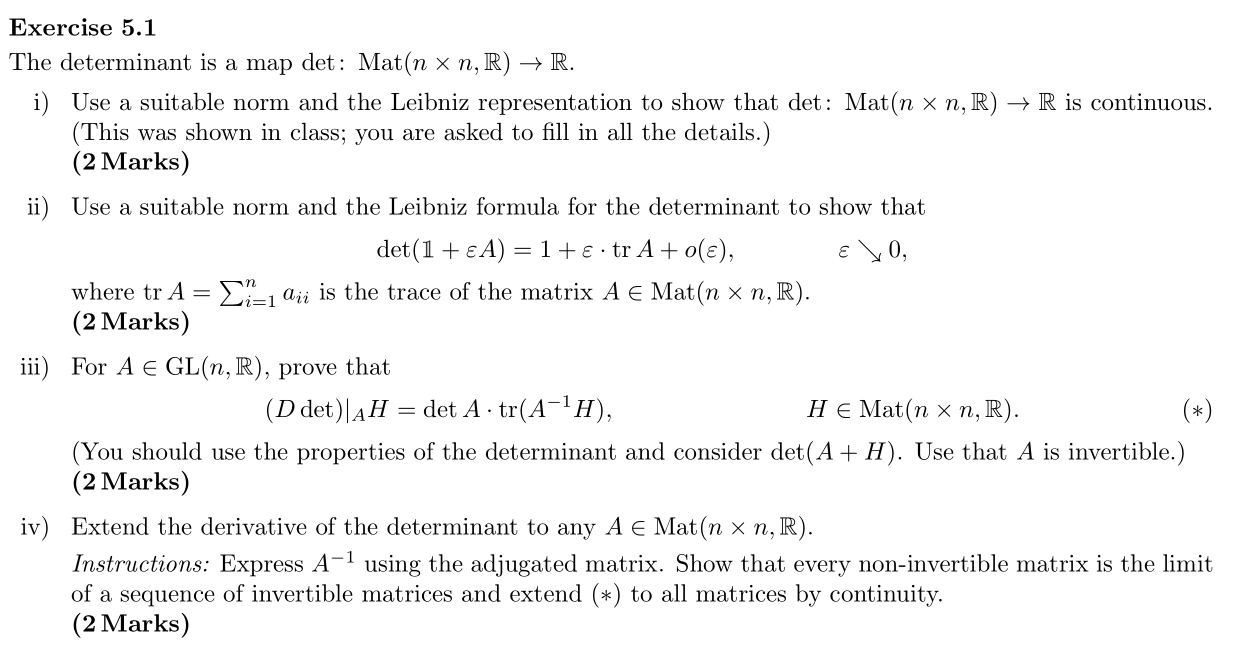
\includegraphics[width=\textwidth]{2020-06-24-23-32-09.png}
    \end{figure}

    \newpage
    i)
    \newpage
    ii)
    \newpage
    iii)
    \newpage
    iv)
    \newpage
    \begin{figure}[H]
        \centering
        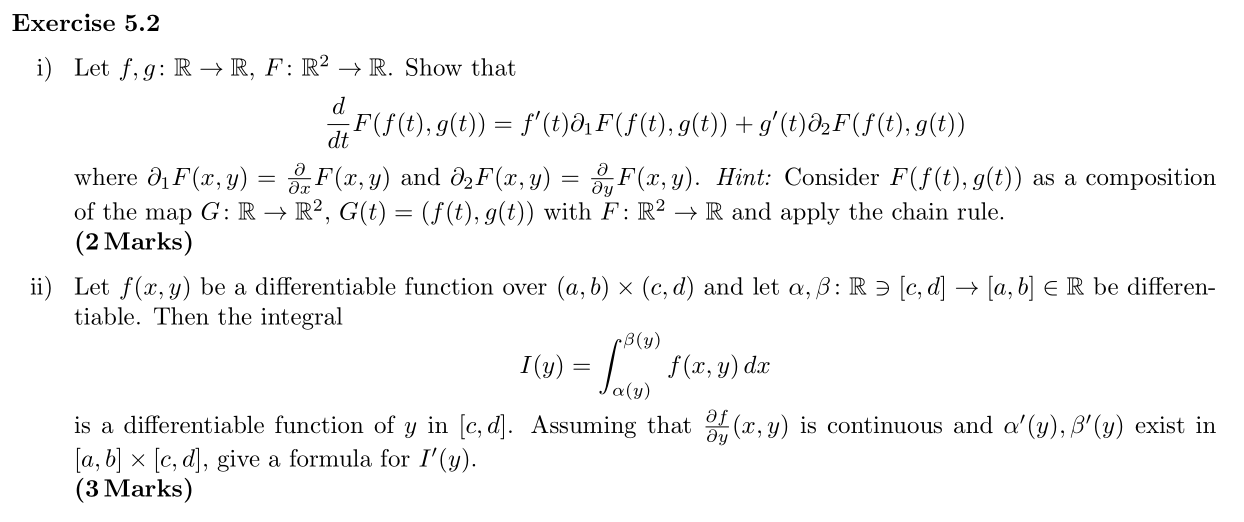
\includegraphics[width=\textwidth]{2020-06-24-23-32-34.png}
    \end{figure}
    \newpage
    i)
    \newpage
    ii)

\end{frame}

\section{First Derivative, Regulated Integral}
\begin{frame}
    \frametitle{Outline}
    \begin{spacing}{1.5}
        \tableofcontents[currentsubsection,hideothersubsections,sectionstyle=hide]
    \end{spacing}
\end{frame}

\begin{frame}
    \frametitle{Something you need to pay attention to...}
    Think More and Be Interactive!
    \begin{itemize}
        \item Do think more about the question in ``()''. \\e.g. ``(How to prove?)''
        \item You are welcome to ask questions in a adequate manner.
        \item Please open your camera so that I can receive more feedbacks from you. (Makes our life easier!)
        \item The class is designed to be interactive. However, if you really do not want to be asked at all, please type an ``\_'' before your zoom name.
    \end{itemize}
\end{frame}

\subsection{Definition of Curves}
\begin{frame}
    \frametitle{Definition of Curves}

    Let $V$ be a finite-dimensional vector space and $I\subset\R$ an interval.
    \begin{itemize}
        \item A set $\mathcal{C}\subset V$ for which there exists a \textbf{continuous, surjective and locally injective} map $\gamma:I\to\mathcal{C}$ is called a \emph{curve}.
        \item The map $\gamma$ is called a \emph{parametrization} of $\mathcal{C}$.
        \item A curve $\mathcal{C}$ together with a parametrization is called a \emph{parametrized} curve.
    \end{itemize}
    \nullspace

    \textbf{Remark:} Curves have several non-equivalent definitions. For example, topological curves, algebraic curves, and what we have learned, parametric curves. Additionally, in majority of the practical cases, we expect our parametrization to be differentiable. We then call these curves differentiable curves.
\end{frame}

\begin{frame}[allowframebreaks]
    \frametitle{Properties of Curves}
    Let $\mathcal{C}\subset V$ be a curve possessing a parametrization $\gamma:I\to\mathcal{C}$ with $\text{int}\,I=(a,b)$ for $-\infty\leq a<b\leq\infty$.
    \begin{itemize}
        \item[(i)] If $\gamma$ is (globally) injective parametrization we say that $\mathcal{C}$ is a \emph{simple curve}. (No intersections)
        \item[(ii)] If \textbf{there exists some $\gamma$}, such that
              \[\lim_{t\to a}\gamma(t)=\lim_{t\to b}\gamma(t),\]
              the curve $\mathcal{C}$ is said to be \emph{closed}.
        \item[(iii)] If a curve is not closed, it is said to be \emph{open}. The points
              \[x:=\lim_{t\to a}\gamma(t)\qquad\qquad\text{and}\qquad\qquad y:=\lim_{t\to b}\gamma(t)\]
              are called the \emph{initial point} and the \emph{final point} of the parametrized curve $(\mathcal{C},\gamma)$. The open curve is said t join $x$ and $y$.
    \end{itemize}
    \newpage
    \Remark Notice the closeness and simpleness of a curve is based on the \textbf{existence} of some parametrization $\gamma$ that meets $(i),(ii)$. If a curve is found to be closed by some parametrization $\gamma$, it is still closed no matter what we choose as a new parametrization.
\end{frame}

\subsection{Orientation of Curves}
\begin{frame}[allowframebreaks]
    \frametitle{Orientation of Curves}
    Let $\mathcal{C}\subset V$ be a curve with parametrization $\gamma:I\to\mathcal{C}$.
    \begin{itemize}
        \item[(i)] Let $J\subset\R$ be an interval. A continuous, bijective map $r:J\to I$ is called a \emph{reparametrization} of the parametrized curve $(\mathcal{C},\gamma)$.
        \item[(ii)] If $r$ is \emph{increasing} the reparametrization is said to be \emph{orientation-preserving}.
        \item[(iii)] If $r$ is \emph{decreasing} the reparametrization is said to be \emph{orientation-reversing}.
    \end{itemize}
    \vspace{1cm}
    Let $(\mathcal{C},\gamma)$ be a parametrized curve and $r$ a reparametrization of $(\mathcal{C},\gamma)$. The curve $(\mathcal{C},\widetilde{\gamma})$ with $\widetilde{\gamma}=\gamma\circ r$ is said to have the \emph{same orientation} as $(\mathcal{C},\gamma)$ if $r$ is orientation-preserving. Otherwise it is said to have \emph{reverse orientation}.
    \newpage
    Only in below case, we can define positive orientation explicitly.\nullspace
    Let $(\mathcal{C},\gamma)$ be a parametrized, simple, closed curve in $\R^2$. Then $\mathcal{C}$ is said to have \emph{positive orientation} if $\gamma$ traverses $\mathcal{C}$ in a \emph{counter-clockwise} direction.
\end{frame}

\subsection{Tangent Vector of Curves}
\begin{frame}[allowframebreaks]
    \frametitle{Tangent Vector of Curves}

    A curve $\mathcal{C}\subset V$ is said to be \emph{smooth} if there exists a parametrization $\gamma:I\to\mathcal{C}$ such that
    \begin{enumerate}[(i)]
        \item $\gamma$ is continuously dif{}ferentiable on $\text{int}\,I$ and
        \item $D\gamma|_t\neq0$ for all $t\in\text{int}\,I$.
    \end{enumerate}
    A \emph{smooth reparametrization} is a reparametrization that is continuously
    dif{}ferentiable with non-vanishing derivative in the interior of its domain.\\[6pt]
    If $V=\R^n$, the Jacobian $D\gamma=\gamma'$ of a smooth curve $\gamma:I\to\R^n$ is given by
    \[\gamma'(t)=\begin{pmatrix}
            \gamma_1'(t) \\
            \vdots       \\
            \gamma_n'(t)
        \end{pmatrix},\qquad\qquad\qquad
        t\in\text{int}\,I.\]

    For smooth curves, we can further define the tangent vectors.\nullspace

    Let $\mathcal{C}^*\subset\R^n$ be an oriented smooth curve and $p\in\mathcal{C}^*$. Let $\gamma:I\to\R^n$ be a parametrization of $\mathcal{C}^*$. Then we define the \emph{unit tangent vector} to $\mathcal{C}^*$ at $p=\gamma(t)$ by
    \begin{equation}\label{2.3.4}
        T\circ\gamma(t):=\frac{\gamma'(t)}{\|\gamma'(t)\|},
        \qquad\qquad\quad t\in\text{int}\,I.
    \end{equation}
    This defines the \emph{tangent vector field} $T:\mathcal{C}^*\to\R^n$ on $\mathcal{C}$. Notice that the unit tangent vector does not depend on the choice of parametrization.\\[5pt]

    \Question Consider the difference between $$T\circ\gamma(t),T\circ\gamma, T,\gamma',\gamma'(t)$$.
\end{frame}

\subsection{Curve Length}
% Natural Parametrization
% Examples
\begin{frame}
    \frametitle{Curve Length}

    We define the \emph{curve length} by
    \[\ell(\mathcal{C}):=\sup\limits_{\text{partitions}\,\mathcal{P}}\ell_\mathcal{P}(\mathcal{C}).\]
    However, in practice, we calculate the curve length by
    \[\ell(\mathcal{C})=\int_{a}^{b}\|\gamma'(t)\|dt\]

    We immediately find that $\ell^{-1}$ is a \emph{natural parametrization} of the curve. i.e., we can
    parametrize $\mathcal{C}$ using
    \[\gamma=\ell^{-1}:I\to\mathcal{C},\qquad
        \qquad\quad\text{int}\,I=(0,\ell(\mathcal{C})).\]
\end{frame}

\begin{frame}
    \frametitle{Exercise}
    In coordinates, we have some function $r=r(\varphi),0<\varphi<2\pi$. Prove its curve length is
    $$
        \ell = \int_0^{2\pi}\sqrt{r^2(\varphi)+r'^2(\varphi)}d\varphi
    $$



\end{frame}

\subsection{Line Integral of a Scalar Function}
% Mention integral of a vector function
% Examples
\begin{frame}
    \frametitle{Line Integral of a Scalar Function}
    The basic idea of the line integral of a scalar function is to calculate ``the total mass of a non-uniform string''.

    Let $\Omega\subset\R^n,f:\Omega\to\R$ be a continuous potential function and $\mathcal{C}^*\subset\Omega$ an oriented smooth curve with parametrization $\gamma:I\to\mathcal{C}$. We then define the \emph{line integral of the potential $f$ along $\mathcal{C}^*$} by
    \[\int_{\mathcal{C}^*}f\,d\ell:=\int_{I}(f\circ\gamma)(t)
        \cdot\|\gamma'(t)\|\,dt\]
    \nullspace
    \Remark The line integral of scalar function (scalar field) does not have many applications in engineering or physics. However, we will soon learn the line integral of vector function, which has many uses in physics.
\end{frame}

\subsection{Normal Vector of Curves, Curvature}

\begin{frame}
    \frametitle{Normal Vector of Curves, Curvature}
    The \emph{unit normal vector} $N:\mathcal{C}\to\R$ is defined by
    \begin{equation}\label{2.3.8}
        N\circ\gamma(t):=\frac{(T\circ\gamma)'(t)}{\|(T\circ\gamma)'(t)\|},
        \qquad\qquad\quad t\in\text{int}\,I.
    \end{equation}

    The \emph{curvature} of a smooth $C^2$-curve $\mathcal{C}\subset V$ is
    \[\kappa:\mathcal{C}\to\R,\qquad\quad
        \kappa\circ\ell^{-1}(s):=\left\|\frac{d}{ds}
        \left(T\circ\ell^{-1}(s)\right)\right\|\]
    where $T$ is the unit tangent vector and $\ell^{-1}:I\to\mathcal{C}$ is the curve length parametrization of $\mathcal{C}$. In fact, we also have\\[5pt]$$\kappa \circ \gamma(t)=\left.\kappa \circ \ell^{-1}(s)\right|_{s=\ell \circ \gamma(t)}=\frac{\left\|(T \circ \gamma)^{\prime}(t)\right\|}{\left\|\gamma^{\prime}(t)\right\|}$$
    Note that, both $N$, $\kappa$ also does not depend on the orientation of $\mathcal{C}$.
\end{frame}

\begin{frame}
    \frametitle{*Curvatrue for Function $y=y(x)$}
    A (twice continuously differentiable) function is a smooth curve, so we can find its curvature.
    $$\kappa=|\dfrac{y''}{(1+y'^2)^{\frac{3}{2}}}|$$
    (You can verify this using the formula of curvature.)
\end{frame}

\begin{frame}[allowframebreaks]
    \frametitle{Exercise: Projectile}
    Let's do some simple physics! Given gravity acceleration $g$. An object with mass $m$ is thrown with an initial velocity $(v_x,v_y)$ from the origin. (Both $v_x,v_y>0$) Find
    \begin{enumerate}
        \item a suitable parametrization.
        \item the trajectory using parametrization.
        \item the length of trajectory before landing.
        \item the curvature of the trajectory at any point.
    \end{enumerate}
    \newpage
    Answer:
\end{frame}

\subsection{*Radius of Curvature}
\begin{frame}
    \frametitle{Extension: Radius of Curvature}
    We can then define the \emph{radius of curvature} by $\kappa$:
    $$\rho:=\dfrac{1}{\kappa}$$
    \begin{figure}[H]
        \centering
        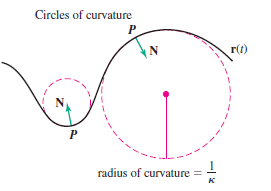
\includegraphics[width=0.4\textwidth]{2020-06-24-22-07-55.png}
    \end{figure}
\end{frame}

\begin{frame}[allowframebreaks]
    \frametitle{Projectile Again}
    Find
    \begin{enumerate}
        \item the radius of curvature of the trajectory at a given point.
        \item the velocity at the same point.
        \item the normal component of the gravitational acceleration at the same point.
        \item what's their relations?
    \end{enumerate}
    \newpage
    Answer:
\end{frame}


\subsection{After Class Exercise}
\begin{frame}
    \frametitle{After Class Exercise}
    Define the parametrization of the cycloid $\gamma(t), t \in(0,2 \pi)$
    \[
        \gamma(t)=\left(\begin{array}{c}
                t-\sin t \\
                1-\cos t
            \end{array}\right)
    \]
    Find the tangent vector, normal vector, curve length function and curvature of this curve.
    $$T \circ \gamma(t)=\left(\begin{array}{c}
                \sin \frac{t}{2} \\
                \cos \frac{t}{2}
            \end{array}\right)        $$
    $$
        N \circ \gamma(t)=\left(\begin{array}{c}
                \cos \frac{t}{2} \\
                -\sin \frac{t}{2}
            \end{array}\right)        $$
    $$
        \operatorname{l}\circ \gamma(t)=4\left(1-\cos \frac{t}{2}\right)
    $$
    $$\kappa \circ \gamma(t)=\frac{1}{4 \sin \frac{t}{2}}
    $$

\end{frame}


\begin{frame}
    \frametitle{About Assignment 6}
    \begin{itemize}
        \item[6.1] \emph{binormal vector} and \emph{torsion}
        \item[6.3] engineering application 
        \item[6.6] \textbf{physics application}, relation (similarity and difference) between maths and physics in line integral. (Very important!) 
    \end{itemize}
    
\end{frame}

\begin{frame}
    \frametitle{Discussion}
    \vspace{1cm}
    \begin{center}
        \LARGE
        Have Fun\\
        And\\
        Learn Well!
    \end{center}
\end{frame}

\end{document}